\paragraph{}
We are going to show that the greedy algorithm is not optimal and as a ratio of 2 with the optimal solution.

\paragraph{}
The Greedy algorithm isn't optimal. The Figure \ref{fig:Diagramme1} shows an input on which an optimal solution uses two unit length intervals, but our greedy algorithm uses three. 

\begin{figure}[h]
	\centering
		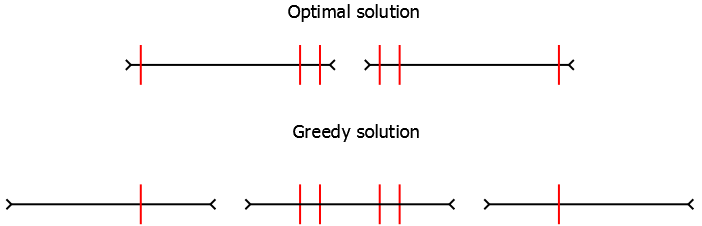
\includegraphics[width=9cm]{Diagramme1.png}
	\caption{Greedy is not optimal}
	\label{fig:Diagramme1}
\end{figure}

\paragraph{}
The Figure \ref{fig:Diagramme2} shows a situation where our greedy algorithm output is as close as we want to 2 times the optimal solution. The idea is to create a lot of singletons that will not be recovered at first ad will result in a lot of overlap at the end. A naive algorithm that recovers all points without overlapping is nearly twice better in this situation.

\begin{figure}[h]
	\centering
		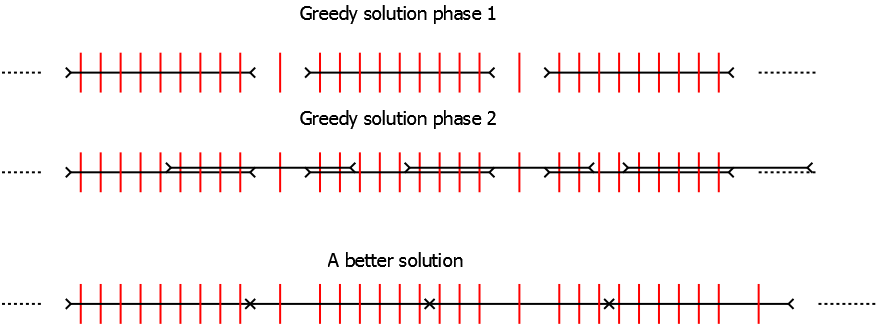
\includegraphics[width=13cm]{Diagramme2.png}
	\caption{Greedy can be 2 times the optimal}
	\label{fig:Diagramme2}
\end{figure}

\paragraph{}
The only thing left is to show that the greedy solution cannot be more than two times worst than the optimal.

\paragraph{}
We first realized that an optimal solution can be found using the simple rule : At all step we choose the interval that start with the leftmost not covered point. The optimality of this algorithm can easily be shown by induction considering an other optimal solution and showing that they use the same number of intervals.

\paragraph{}
We also consider a slightly different algorithm than the greedy. It chooses the same intervals except that it always puts a not-yet-covered point at the left extreme of the interval. This other version of the greedy algorithm builds the exact same number of interval.

\paragraph{}
We now want to show that our greedy algorithm does not use more than two times the number of intervals used above. We first show that any point cannot be covered by more than 2 intervals. This is illustrated by Figure \ref{fig:Diagramme3}. The interval 1 cannot be chosen after 2 or 3 because we follow the above rule, neither can 2 after 3. Furthermore 3 will always be chosen before 2 because 3 contains more uncovered points.

\begin{figure}[h]
	\centering
		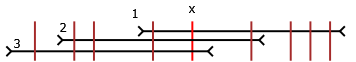
\includegraphics[width=9cm]{Diagramme3.png}
	\caption{Greedy is not optimal}
	\label{fig:Diagramme3}
\end{figure}


